\section{Evaluation} \label{sec:eval}

The evaluation of the Page Rank simulation framework will comprise of two steps. First of all, we will give a brief overview of some benchmarking considerations - see section \ref{sec:bench}. Then, the first stage will focus on tuning the simulation parameters, which define the time allowance given to a Page Rank iteration to execute - see section \ref{sec:partun}. The second stage will demonstrate the performance achieved by SpiNNaker, first under varying placement conditions and then relative to a Python implementation of Page Rank - see section \ref{sec:perf}. \\

\subsection{Benchmarking  considerations} \label{sec:bench}

A key feature of these benchmarks is the parameters chosen to modulate the running time of a simulation. Considering a Page Rank graph that needs 10 iterations to converge, then two configuration parameters can influence its wall-clock time:

\begin{itemize}
\item \textbf{time\_step} (ms): hardware clock time between each timer tick. The bigger this time step the more time the core has between each timer tick.
\item \textbf{time\_scale\_factor} (unit-less): scales up the wall-clock execution time, by slowing down the notion of time on SpiNNaker by some factor. 
\end{itemize}

The table below illustrates the implications of different configurations of these parameters on the number of timer ticks and on the wall-clock running time.

\begin{center}
\begin{tabular}{ |c|c|c|c|c| }
 \hline
 sim. time & \texttt{time\_step} & \texttt{time\_scale\_factor} & \textbf{timer ticks} & \textbf{wall-clock time}  \\ 
 \hline
10 & 1 & 1 & 10 & \textbf{10} \\ 
10 & 2 & 1 & 5 & \textbf{10} \\ 
10 & 1 & 2 & 10 & \textbf{20} \\ 
 \hline
\end{tabular}
\end{center} 

This level of granularity between wall-clock execution time and SpiNNaker time was required by spiking neural networks simulations, but is not useful for Page Rank. Indeed, synapsic model can be time-based whereas Page Rank iterations do not have any such dependence. Consequently, we will be fixing the \texttt{time\_step} during this evaluation and varying the \texttt{time\_scale\_factor} to modulate the running time of Page Rank simulations. \\

Another relevant detail to note is that it seems hazardous to compare the raw running times of two machines of such different natures, such a a neuromorphic and a traditional personal computer. Therefore, all the comparisons we make will be based on arbitrary-unit running times and the point of interest will be the scaling trends of one machine versus the other. Other running times that do not involve cross-machine comparisons will be expressed in \texttt{time\_scale\_factor}, taking a constant simulation time throughout the entire evaluation. Hence, only the \texttt{time\_scale\_factor} defines the \textit{wall-clock} simulation time in that setting. The simulation time chosen is $2.5ms$, with the default \texttt{time\_step} of $0.1ms$ \cite{defts}, giving 25 timer ticks; hence up to 25 iterations for Page Rank. As we are not interested in Page Rank convergence here, we always run the 25 iterations of Page Rank to be able to compare the running times of different graphs. \\

Finally, let us recall several graph topology considerations to disambiguate any magical number used in this benchmark. To begin with, we use 10 edges for each vertex to maximise network usage (explained in \ref{sec:resval}). Additionally, it is important to remember that a SpiNNaker core manages 255 vertices by default, and each chip contains $15 \times 255 = 3,825$ vertices; the last application core being used to re-inject dropped packets. Also, the Spin3 (see Fig.~\ref{fig:spin3}), which we use for these tests, contains 4 SpiNNaker chips so the maximum number of vertices we can simulate is $4 \times 3,825 = 15,300$. \\

\subsection{Parameter tuning} \label{sec:partun}

When SpiNNaker is not allowed enough time to process packets during an each iteration, it starts dropping packets. This can occur at two different layers: (a) at the network layer with router buffers overflowing or (b) at the core level which is not allowed enough time to process the entire incoming workload.

\begin{figure}[!ht]
    \centering
    \begin{subfigure}[b]{0.5\textwidth}
        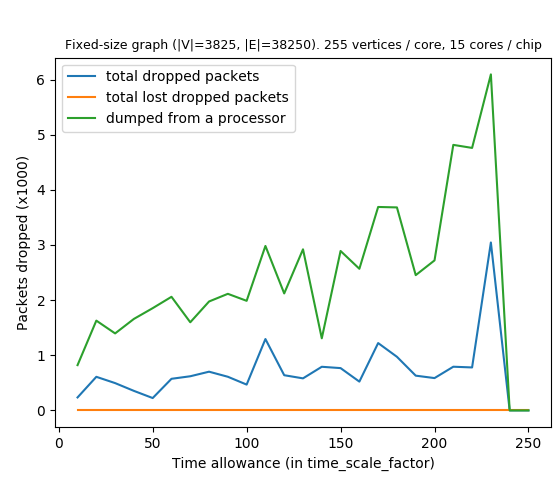
\includegraphics[width=\textwidth]{figures/packet_drop_vs_time_scale_factor-1.png}
        \caption{} \label{fig:graph11}
    \end{subfigure}%
    ~ %add desired spacing between images, e. g. ~, \quad, \qquad etc.
      %(or a blank line to force the subfigure onto a new line)
    \begin{subfigure}[b]{0.5\textwidth}
        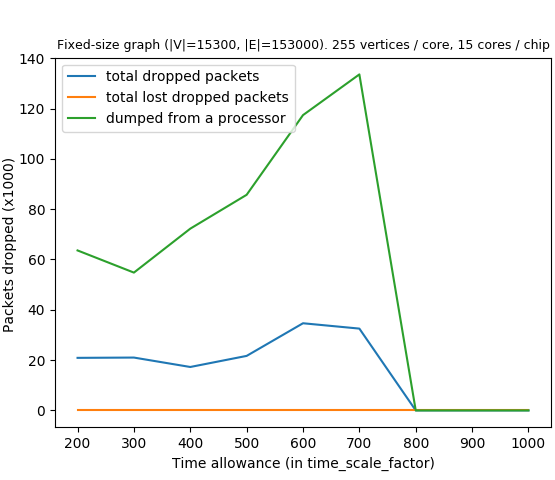
\includegraphics[width=\textwidth]{figures/packet_drop_vs_time_scale_factor-2.png}
        \caption{} \label{fig:graph12}
    \end{subfigure}
    \caption{Tuning hardware time step to avoid dropping packets}
    %\caption{Minimising simulation running time while preventing packet drops}
    \label{fig:graph1}
\end{figure} 

In Fig.~\ref{fig:graph1}, we show an attempt to minimise the simulation running time while preventing packet drops for two sizes of graph. The first graph in Fig.~\ref{fig:graph11} fills an entire chip ($3,825$ vertices) and increases the \texttt{time\_scale\_factor} iteratively, while the second graph in Fig.~\ref{fig:graph12} fills all four chips of the board ($15,300$ vertices). For the first graph, we can note that $\texttt{time\_scale\_factor} = 230$ is the value from which Page Rank has enough time to be computed successfully, while this number is below $800$ for a bigger graph. Already, we can see that for 4 times the graph size (4 chips vs. 1 chip), the running time is only multiplied by $800/230 = 3.5$. This is a positive scaling result for an algorithm, Page Rank, that has a complexity of $O(|V|+|E|)$ that is linear in the sum of vertices and edges. \\

Maybe surprisingly, we note as a general trend that the more time we allow for execution, the more packets get dropped. This is due to the number of packets sent also increasing with \texttt{time\_scale\_factor}. Indeed, less time meant cores got interrupted before even sending all of their packets. \\

A second takeaway from these graphs is certainly the comparison between the two sources of bottlenecks: network usage \& core processing. On both graph sizes, the number of packets dropped by cores (green curve) increases faster than the number of packets dropped by the network (blue curve). Moreover, absolutely all packets dropped by the network get successfully re-injected in the network, as indicated by the flat orange curve at $y=0$. This indicates the cores are the main bottleneck of the computation. To keep the same processing capabilities in terms of graph size, the Page Rank framework code running on the cores could be made more efficient. However, the existing implementation, which is based on the partly-optimised neuron implementation of \texttt{sPyNNaker}, is already relatively optimised and might not have a lot of speed-up potential left to exploit. Another option is to reduce the number of vertices that a single core manages. The latter is an option that will be covered in the next section \ref{sec:perf}, but we can already note its main drawback is the reduced capability in terms of graph size input. Indeed, if $15,300$ vertices already filled up the entire board, then dividing by half the number of vertices per core would also divide by half that maximum capacity of $15,300$ down to $7,650$ vertices. \\

This now leads us to the second stage of this evaluation, where we will be covering the performance achieved by this project after porting Page Rank to SpiNNaker. \\

\subsection{Performance measure} \label{sec:perf}

\subsubsection{Resources vs. performance trade-off}

This first preliminary benchmark is interested in the performance trade-off mentioned earlier, where running time and resource utilisation oppose each other. Indeed, less vertices managed by core means poorer resource utilisation, so let us see to what extent it gives better running times that would justify compromising on resources - see Fig.~\ref{fig:graph2}.

\begin{figure}[!ht]
    \centering
    \begin{subfigure}[b]{0.5\textwidth}
        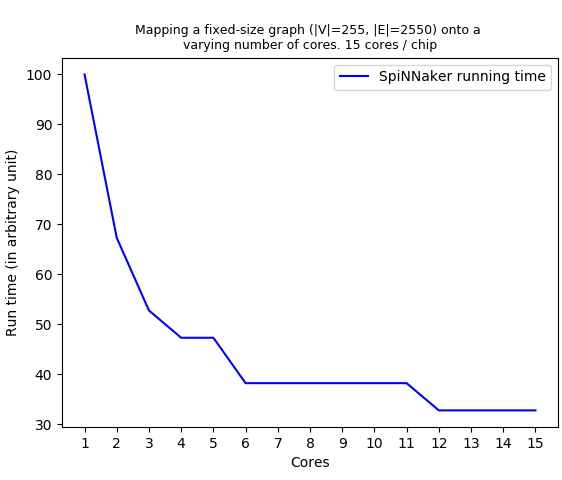
\includegraphics[width=\textwidth]{figures/atoms_per_core_vs_running_time-1.png}
        \caption{} \label{fig:graph21}
    \end{subfigure}%
    ~ %add desired spacing between images, e. g. ~, \quad, \qquad etc.
      %(or a blank line to force the subfigure onto a new line)
    \begin{subfigure}[b]{0.5\textwidth}
        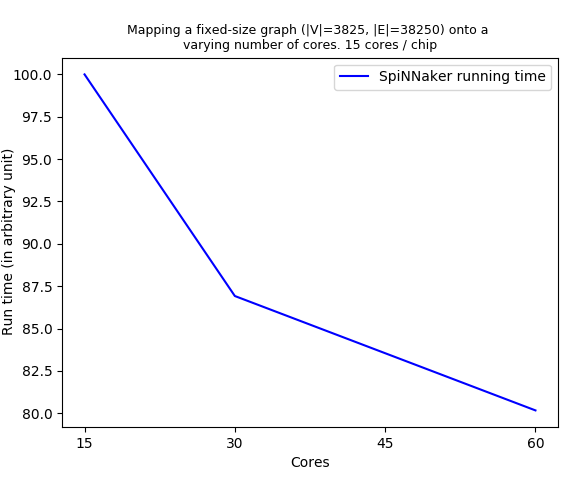
\includegraphics[width=\textwidth]{figures/atoms_per_core_vs_running_time-2.png}
        \caption{} \label{fig:graph22}
    \end{subfigure}
    \caption{Tuning number of Page Rank vertices managed by a single core}
    %\caption{Trade-off between running time and resource utilisation}
    \label{fig:graph2}
\end{figure} 

In Fig.~\ref{fig:graph2}, the first graph \ref{fig:graph21} takes a fixed-size graph that fits on a single core, which is then partitioned into a varying number of cores. In practice, this is done by setting a constant at runtime that defines how many vertices of the graph should be mapped by \texttt{PACMAN} to a single core. Here, it is quite clear that the greater the number of nodes for the same graph, the better the running time is. However, this trend seems to tapper off from 6 cores onwards. For example, splitting this graph between 4 cores, managing $255 / 4 \approx 64$ vertices each, reduces the running time by more than half. \\

However on the second graph \ref{fig:graph22}, a similar trend is observed but to a lesser extent. Indeed, when quadrupling the number of cores used for the simulation (from 15 to 60), the running time is only reduced by $-20\%$ (from $100$ down to $80$) whereas it decreased by over $-50\%$ in the first case. This is due to: (a) the network overhead of a larger graph and (b), the added cost of chip-to-chip communication, which was not present in the previous case where all cores were on the same chip. \\

All in all, this experiment encourages SpiNNaker users to divide their graphs so that they are mapped to as many cores as possible and make full use of the hardware capabilities of the machine. This also shows this network load could be reduces by a clever partitioning of graph that minimises the chip-to-chip communication overhead.

\subsubsection{Performance at scale}

Finally, this last experiment is the most important one as is compares the scaling potential of Page Rank on SpiNNaker versus an implementation running on a traditional PC. For the Python implementation, we use an adapted version of the Page Rank algorithm from the \texttt{networkx} \cite{networkx} network manipulation library. The trace of running times of both machines are normalised relative to their first value, so that both scaling curves have the same starting point - see Fig.~\ref{fig:graph3}. These arbitrary units make the Core Processing Unit (CPU) model of the PC used irrelevant, as the scaling curve will have the same shape no matter how fast it runs on a given CPU.

\begin{figure}[!ht]
    \centering
    \begin{subfigure}[b]{0.5\textwidth}
        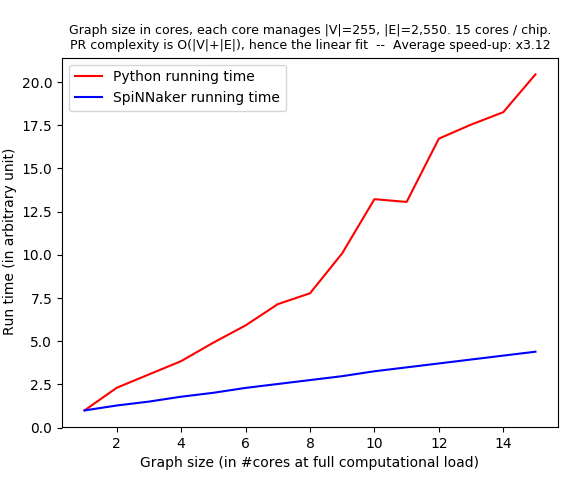
\includegraphics[width=\textwidth]{figures/graph_size_vs_running_time-1.png}
        \caption{} \label{fig:graph31}
    \end{subfigure}%
    ~ %add desired spacing between images, e. g. ~, \quad, \qquad etc.
      %(or a blank line to force the subfigure onto a new line)
    \begin{subfigure}[b]{0.5\textwidth}
        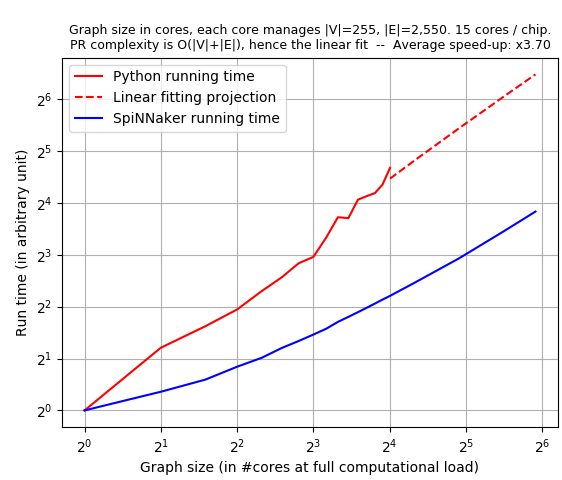
\includegraphics[width=\textwidth]{figures/graph_size_vs_running_time-2.png}
        \caption{} \label{fig:graph32}
    \end{subfigure}
    \caption{Page Rank (PR) scalability of Python vs. SpiNNaker}
    %\caption{Page Rank linear scaling on different architectures}
    \label{fig:graph3}
\end{figure} 

First of all, we observe on both graphs that the scaling curves are approximately linear, which is consistent with the complexity $O(|V|+|E|)$ of Page Rank that remains unchanged. In Fig.~\ref{fig:graph31}, we see how both implementations scale on a graph that gradually fits up to an entire chip, that is $3,825$ vertices and ten times more edges. We also observe SpiNNaker brings a significant speed up in terms of scaling trend, averaged at a factor of x$3.12$ (see figure title). Likewise in Fig.~\ref{fig:graph32}, SpiNNaker clearly outperforms the traditional PC at a comparable speed-up factor of $3.70$ when scaling to larger graph sizes. Last but not least, for the last data point of the graph at $x=60$, the speed-up obtained is around $5$ while it is smaller for the first data points. This reveals that the scaling potential of SpiNNaker is not constant compared to the PC, but rather that it increases with larger graph sizes which is another positive contribution. \\

Overall, this evaluation confirms Page Rank on SpiNNaker has a significant scaling potential compared to a standard implementation running on a PC. It also shed light on the bottleneck of the current implementation, which is the heavy workload processed by cores. This leaves some further scaling opportunities for a follow-up project that would optimise the current Page Rank framework and potentially generalise it to other graph-based algorithms with comparable data flows. Lastly, it is interesting to see how efficient packet re-injection is. A better implementation on the processing cores that would push the bottleneck to the network could always lower the threshold from 0 packet dropped to 0 lost dropped packet (see Fig.~\ref{fig:graph1}). \\

\textit{Nota bene}: all the scripts used to run this benchmark can be found in the examples folder of the project folder, under \texttt{python/page\_rank/examples/plot\_*.py}.

\subsection{Limitations} \label{sec:lim}

Nonetheless, the implementation also has its limits which might discourage real-life graph processing applications of SpiNNaker. Firstly, the input size accepted by this implementation is limited by the hardware used. As show in the results above, the largest graph that can run on the Spin3 chip contained $15,300$ vertices. Even when using the biggest version of the machine, we would still not be able to process the largest graphs from Google or Facebook. Indeed, that machine has $1,036,800 cores$, of which only $15/18$ run the application code of the simulation, meaning the maximum number of vertices we could accept would be: $1,036,800 \times 15 \ 18 \times 255 = 220M$. With such capacities, SpiNNaker cannot compete with very large scale graph processing tools. \\

Moreover, the start-up time of simulations was not taken into account here. Indeed, the vast majority of the time is spent pre-processing the graph, the main bottleneck being the construction of the data specification which is loaded on SpiNNaker. Only long running algorithms would justify the upfront cost required by this pre-processing stage, and Page Rank usually converges in a few hundreds of iterations, which get computed relatively fast. Large graph inputs should be benchmarked to confirm if the start-up cost can be compensated by the running time speed-up on SpiNNaker. \\

This perfectly introduces one of the problems of this evaluation, which is that it only ran on small machine. Although the results are encouraging for larger graphs, only a proper testing phase on a bigger machine could confirm the true scalability potential of this Page Rank simulation framework. This would also allow for the asynchronous model to be tested, as it is more likely iterations will get out of synchronisation on a bigger input graph mapped to a large number of cores.

%Additionally, someone could critique the lack of diversity of graph topologies for this evaluation. !!!!!
%
%
%evaluation is not complete some further tests would be required to confirm the scaling potential 
%
%- Async implementation should be demonstrated at scale
%- No graph benchmarking, dense graph to maximise network usage. Should be confirmed by the graph generation step of a graph bencharming algorithm
%tried on dense graph with uniform edge repartition.

\newpage
%% - MCMC approximates results, we have the exact results fixed-point ARM9 cores
%
%
%Over the course of the project, the measure of success will be defined in the following way:
%
%\begin{enumerate}
%\item \textbf{Neuromorphic-friendly problems}: the core objective and stepping stone to further work will rely on identifying a class of algorithmic problems that are more efficiently solved on neuromorphic hardware, such as SpiNNaker, compared to regular computers.
%
%Benchmarking such a system will be a non-trivial task and supposes we answer several questions: how do we compare performance on neuromorphic versus regular hardware? What weight do we give running time, hardware upfront cost (buying it), hardware operating cost (operating it, i.e. power consumption) in our measure of performance? To answer these questions, we will be using inspiration from the following papers:
%
%\begin{itemize}
%\item Testing the SpiNNaker hardware in its early stages using the NEST spiking neural network simulator with similar computational resources. \cite{bench-spinnaker}
%
%\item The GAP benchmark suite that aims to standardise how graph processing techniques compare to each other. \cite{bench-gap}
%
%\item Benchmarking approach used for Markov chain Monte Carlo sampling on graphical models on the SpiNNaker neuromorphic architecture. \cite{markov-on-spinn}
%
%\end{itemize}
%
%
%\item \textbf{Supporting SpiNNaker library}: building on the first milestone, the second step consists in developing a set of tools that will ease how this class of problems is ported to the SpiNNaker event-driven paradigm. Success will first rely on functional soundness and operability of the library, but will also have a focus on developer experience and ease of use. It should define a clear, simple, flexible and extensible API that would make it a reliable and useful tool for application developers.
%
%Furthermore, depending on timing and how successful this tool is, there is always room to accomplish more to getting in touch with the SpiNNaker software development team and investigate opportunities of collaboration related to my project. If it works well, they could potentially be interested in integrating it to their code base. That would be the most satisfactory outcome and would demonstrate the total success of the project.
%
%\end{enumerate}